% 图 B.4 磁学边界条件：跨越界面的扁盒高斯面（B 垂直分量）与安培环路（H 平行分量）
\documentclass[tikz,border=5pt]{standalone}
\usetikzlibrary{arrows.meta}
\usepackage{amsmath}
\usepackage{bm}
\usepackage{fontspec}
\setmainfont{Times New Roman}
\begin{document}
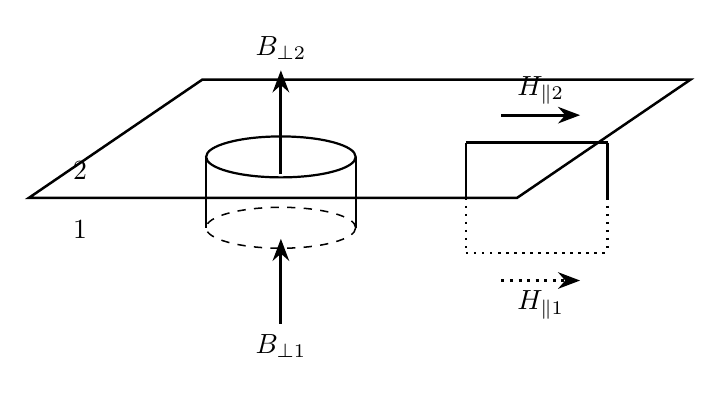
\begin{tikzpicture}[line width=0.8pt,>=Stealth]
% ---------- interface ----------
\draw[line width=0.9pt] (-3.9,0) -- (2.3,0) -- (4.5,1.5) -- (-1.7,1.5) -- cycle;
\node at (-3.25,0.35) {$2$};
\node at (-3.25,-0.40) {$1$};
% ---------- pillbox Gaussian surface (left) ----------
\begin{scope}[shift={(-0.7,0)}]
  \draw[line width=0.6pt] (-0.95,-0.38) -- (-0.95,0.52);
  \draw[line width=0.6pt] (0.95,-0.38) -- (0.95,0.52);
  \draw[dashed,line width=0.55pt] (0,-0.38) ellipse (0.95 and 0.26);
  \draw[line width=0.8pt] (0,0.52) ellipse (0.95 and 0.26);
  % normal component arrows
  \draw[line width=1.1pt,->] (0,0.30) -- (0,1.62);
  \node[above] at (0,1.62) {$B_{\perp 2}$};
  \draw[line width=1.1pt,->] (0,-1.60) -- (0,-0.52);
  \node[below] at (0,-1.60) {$B_{\perp 1}$};
\end{scope}
% ---------- rectangular Amperian loop (right) ----------
\begin{scope}[shift={(2.55,0)}]
  \draw[line width=0.9pt] (-0.9,0.70) -- (0.9,0.70);
  \draw[line width=0.9pt] (-0.9,0.70) -- (-0.9,0);
  \draw[line width=0.9pt] (0.9,0.70) -- (0.9,0);
  \draw[dotted,line width=0.9pt] (-0.9,0) -- (-0.9,-0.70);
  \draw[dotted,line width=0.9pt] (0.9,0) -- (0.9,-0.70);
  \draw[dotted,line width=0.9pt] (-0.9,-0.70) -- (0.9,-0.70);
  % parallel component arrows
  \draw[line width=1.1pt,->] (-0.45,1.05) -- (0.55,1.05);
  \node[above] at (0.05,1.05) {$H_{\parallel 2}$};
  \draw[dotted,line width=1.1pt,->] (-0.45,-1.05) -- (0.55,-1.05);
  \node[below] at (0.05,-1.05) {$H_{\parallel 1}$};
\end{scope}
\end{tikzpicture}
\end{document}
